\chapter{Koncepcja pracy}

\section{Wymagania projektowe}

Końcowym celem projektu jest poznanie procesów kluczowych w internetowych transmisjach audio-wideo
oraz wykonanie aplikacji aplikacji okienkowej na systemy Linux pełniącej rolę komunikatora
internetowego. Komunikator powinien pozwalać użytkującym go użytkownikom na odkrywanie innych
użytkowników i prowadzenie z nimi połączeń audio-wideo. Połączenia audio-wideo pomiędzy
użytkownikami będą odbywać się w trybie peer-to-peer, tj. transmisje wideo i audio w tych
połączeniach trafiają na drugą stronę połączenia bezpośrenio, bez pośrednictwa serwera, który będzie
służył tylko i wyłącznie do dwóch celów: by umożliwiać użytkownikom odkrywanie innych dostępnych
użytkowników do których można wykonać połączenie, oraz jako mechanizm początkowej wymiany danych
pomiędzy stronami połączenia celem sygnalizacji połączenia oraz późniejszego ustanowienia
bezpośredniego kanału wymiany danych peer-to-peer.

\section{Wymagania funkcjonalne}

\begin{enumerate}
	\item Użytkownik może wybrać imię pod którym widoczny będzie dla innych użytkowników
	\item Użytkownik widzi listę aktualnie dostępnych użytkowników
	\item Użytkownik X może zadzwonić do użytkownika Y
	\item Użytkownik X w trakcie oczekiwania na odpowiedź od użytkownika Y, może zrezygnować z
	      połączenia, rozłączyć się
	\item Użytkownik Y, gdy dzwoni do niego użytkownik X, może odrzucić lub odebrać połączenie
	\item Jeśli połączenie zostanie odebrane i poprawnie nawiązane, każdy z użytkowników powinien
	      móc zaobserwować transmisję z kamery wideo oraz usłyszeć transmisję audio z mikrofonu
	      drugiego użytkownika
	\item W trakcie trwania połączenia, każdy z użytkowników może rozłączyć się, unilateralnie
	      terminując połączenie.
\end{enumerate}

\section{Wymagania niefunkcjonalne}

\begin{enumerate}
	\item Do realizacji projektu zostanie wykorzystany język programowania Rust
	\item Aplikacja wykorzystuje frameworki i biblioteki natywne dla systemów Linux
	\item Aplikacja powinna działać nie tylko w sieci lokalnej, ale także w sieci Internet
	\item Aplikacja wykorzystuje kodek AV1 do kompresji wideo
	\item Aplikacja powinna wdzięcznie obsługiwać brak kamery wideo lub mikrofonu przez użytkownika
	\item Połączenia pomiędzy użytkownikami powinny odbywać się w trybie peer-to-peer celem
	      minimalizacji opóźnień
	\item Z powodu powyższego wymagania, połączenia są ograniczone do dwóch użytkowników, tj. nie ma
	      możliwości tworzenia konferencji z wieloma użytkownikami.
\end{enumerate}

\chapter{Zagadnienia teoretyczne}

\section{Kodowanie wideo}


\url{https://github.com/leandromoreira/digital_video_introduction#basic-terminology}

\subsection{Podstawy}

An image can be thought of as a 2D matrix. If we think about colors, we can extrapolate this idea
seeing this image as a 3D matrix where the additional dimensions are used to provide color data.

If we chose to represent these colors using the primary colors (red, green and blue), we define
three planes: the first one for red, the second for green, and the last one for the blue color.

We'll call each point in this matrix a pixel (picture element). One pixel represents the intensity
(usually a numeric value) of a given color. For example, a red pixel means 0 of green, 0 of blue and
maximum of red. The pink color pixel can be formed with a combination of the three colors. Using a
representative numeric range from 0 to 255, the pink pixel is defined by Red=255, Green=192 and
Blue=203.

\subsection{Mechanizmy kompresji}

\subsubsection{Chroma subsampling}

Our eyes are more sensitive to brightness than colors. With the image represented as luma and chroma
components, we can take advantage of the human visual system's greater sensitivity for luma
resolution rather than chroma to selectively remove information. Chroma subsampling is the technique
of encoding images using less resolution for chroma than for luma.

\begin{figure}[H]
	\centering
	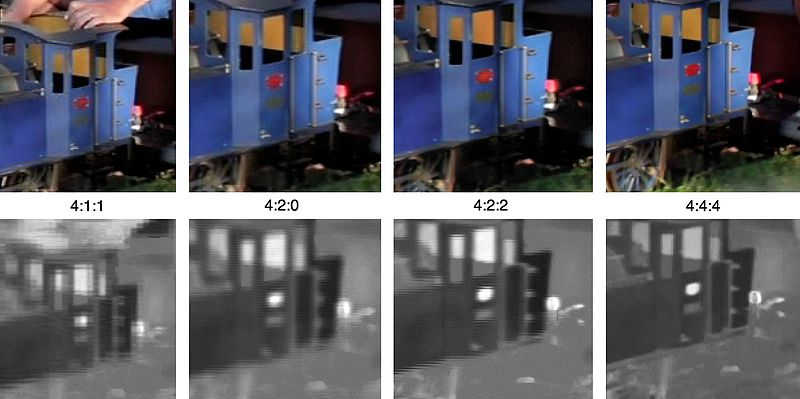
\includegraphics[width=\textwidth]{img/rozdzial2/chroma_subsampling_examples}
	\caption{Przykład różnych typów chroma subsampling. Pomimo bardzo niskiego próbkowania informacji o kolorze, w górnym rzędzie nie widać znaczących różnic pomiędzy pierwszym i ostanim obrazkiem.}
\end{figure}

Now we can move on and try to eliminate the redundancy in time.

\subsection{Inter-frame coding}

Inter-frame coding is reusing information between frames.

Let's explore the options we have to reduce the repetitions in time, this type of redundancy can be solved with techniques of inter prediction.

We will try to spend fewer bits to encode the sequence of frames 0 and 1.

\begin{figure}[H]
	\centering
	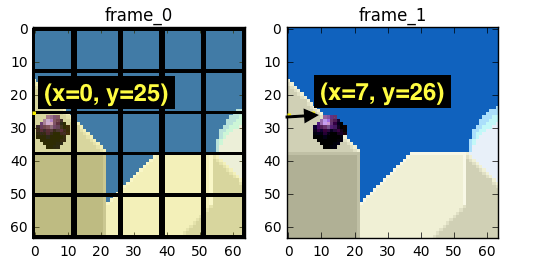
\includegraphics[width=.5\textwidth]{img/rozdzial2/original_frames_motion_estimation}
\end{figure}

One thing we can do it's a subtraction, we simply subtract frame 1 from frame 0 and we get just what we need to encode the residual.

\begin{figure}[H]
	\centering
	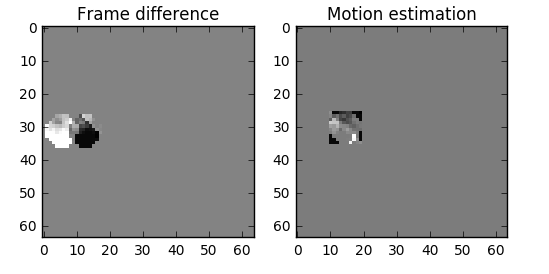
\includegraphics[width=.5\textwidth]{img/rozdzial2/difference_frames}
\end{figure}

But what if I tell you that there is a better method which uses even fewer bits?! First, let's treat the frame 0 as a collection of well-defined partitions and then we'll try to match the blocks from frame 0 on frame 1. We can think of it as motion estimation.

Also motion vectors.

\subsection{Intra-frame coding}

If we analyze each frame in a video we'll see that there are also many areas that are correlated.

\begin{figure}[H]
	\centering
	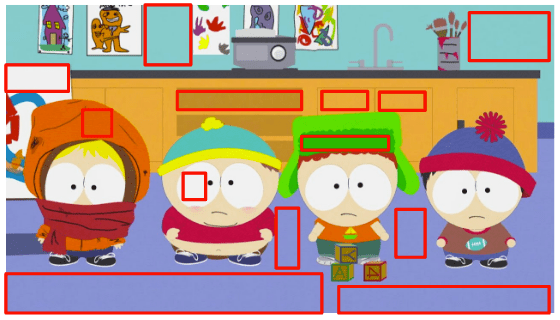
\includegraphics[width=.5\textwidth]{img/rozdzial2/repetitions_in_space}
\end{figure}

\subsection{Standardy kodowania}
\subsubsection{Podstawy}
\subsubsection{AVC}

AVC jest standardem kodowania wideo przyjętym w roku 2003 przez MPEG. Jego najpopularniejszą
implementacją jest biblioteka x264.

\subsubsection{AV1}

\section{Internetowe strumienie wideo}

Jakieś wprowadzenie o wideo ogólnie, w jakich kontekstach występuje (pliki wideo, streaming np. Youtube/Netflix,
strumienie czasu rzeczywistego np. Twitch/Discord/Teams), czym te konteksty się różnią.

Możemy wyróżnić 3 rodzaje wideo:

\begin{itemize}
	\item lokalne pliki wideo - pliki wideo na dysku w kontenerze mp4, mkv, lub innym
	\item streamowanie plików wideo (np. Youtube albo Netflix) - mamy przygotowane segmenty pliku
	      wideo w różnych rozdzielczościach i wysyłamy je po kolei, dobieramy rozdzielczość wg.
	      dostępnego pasma pomiędzy serwerem a klientem
	\item strumieniowanie w czasie rzeczywistym - priorytetem jest opóźnienie, kodujemy na bieżąco
	      przechwytywane klatki i wysyłamy je najszybciej jak się da; przez to niektóre mechanizmy
	      kompresji są niedostępne (np. B-klatki, które wykorzystują dane z następnej klatki aby
	      zmniejszyć wielkość klatki)
\end{itemize}

Zidealizowany obraz rozmowy wideo w internecie:
\begin{enumerate}
	\item Komputery są publicznymi hostami w internecie i program komunikatora słucha na danym porcie
	\item Strona nawiązująca połączenie łączy się do hosta odbiorcy po tym porcie, sygnalizuje chęć
	      nawiązania połączenia
	\item Strona odbierająca akceptuje
	\item Kamera oraz mikrofon nadawcy przechwytują najlepszy możliwy obraz i dzwięk, i przesyłają
	      je do komputera
	\item Strumienie wideo i audio są łączone i synchronizowane
	\item Komputer wysyła strumień audio-wideo wcześniej ustanowionym kanałem
\end{enumerate}

Natomiast pojawiają się problemy:

\begin{enumerate}
	\item Komputery znajdują się w sieciach domowych, za NATem, nie można się do nich bezpośrednio
	      połączyć
	\item Nieskompresowane wideo jest zbyt duże by wysłać je przez internet, potrzebny jest jakiś
	      mechanizm kompresji
	\item Komputery mogą mieć różne możliwości przetwarzania wideo: znajdować się w sieciach o
	      znacząco różnej szybkości, mieć różniące się szybkością procesory, kamery zapisujące
	      klatki w różnych formatach
\end{enumerate}

W następnym rozdziale zaprezentowane zostaną technologie rozwiązujące powyższe problemy.
